\documentclass[a4paper, UKenglish, cleveref, autoref, thm-restate]{lipics-v2021}

\usepackage{amsmath}
\usepackage{prooftree}
\usepackage{tikz}

\bibliographystyle{plainurl}

\newcommand{\fall}[1]{\forall{#1}.}
\newcommand{\lam}[1]{\lambda{#1}.}

\title{All watched over by machines of loving grace}
\titlerunning{Supervisionary system description}

\ccsdesc{}
\keywords{Proof assistant design, operating systems, LCF, Supervisionary, capabilities}

\author{Dominic P. Mulligan}{Automated Reasoning Group, Amazon Web Services\footnote{All work done whilst at Arm Research} \and \url{www.dominic-mulligan.co.uk}}{dominic.p.mulligan@gmail.com}{}{}
\authorrunning{Dominic P. Mulligan}

\Copyright{Dominic P. Mulligan}

\acknowledgements{}

\begin{document}

\maketitle

\begin{abstract}
Modern operating systems are typically built around a trusted system component called the \emph{kernel} which amongst other things is charged with enforcing system-wide security policies.
Crucially, this component must be kept isolated from untrusted software at all times, which is facilitated by exploiting machine-oriented notions of separation: private memories, privilege levels, and similar.

Modern proof-checkers are typically built around a trusted system component called the \emph{kernel} which is charged with enforcing system-wide soundness.
Crucially, this component must be kept isolated from untrusted automation at all times, which is facilitated by exploiting programming-language notions of separation: module-private data structures, type-abstraction, and similar.

Whilst markedly different in purpose, in some essential ways operating system and proof-checker kernels are tasked with the same job, namely enforcing system-wide invariants in the face of unbridled interaction with untrusted code, yet the mechanisms through which the two types of kernel protect themselves are significantly different.
In this paper, we introduce \emph{Supervisionary}, a prototype programmable proof-checking system for Gordon's HOL that is organized in a manner more reminiscent of operating systems than typical LCF-style proof-checkers.
In particular, Supervisionary implements a kernel that executes at a relative level of privilege compared to untrusted automation, with trusted and untrusted system components communicating across a limited system call boundary to indirectly manipulate kernel objects managed by the Supervisionary kernel via handles.

Unusually, Supervisionary has no ``metalanguage'' in the LCF sense, as the language used to implement the kernel, and the language used to implement automation, need not be the same.
Indeed, \emph{any} programming language can be used to implement automation for Supervisionary providing the resulting binary respects the Supervisionary kernel calling convention and binary interface, with no risk to system soundness.
Moreover, we observe that Supervisionary allows arbitrary programming languages to be endowed with facilities for proof-checking, not only dedicated languages like Idris and Agda.
Indeed, the handles that Supervisionary uses to reference kernel objects under its management may be thought of as a form of \emph{capability}, in the hardware sense.
However, unlike typical capabilities, Supervisionary's capabilities are extremely expressive, essentially capturing the full expressive power of HOL, and could be used to enforce fine-grained correctness and security properties at runtime.
\end{abstract}

\section{Introduction}
\label{sect.introduction}

\subsection{On operating systems}

\begin{figure}
\tikzset{every picture/.style={line width=0.75pt}} %set default line width to 0.75pt        
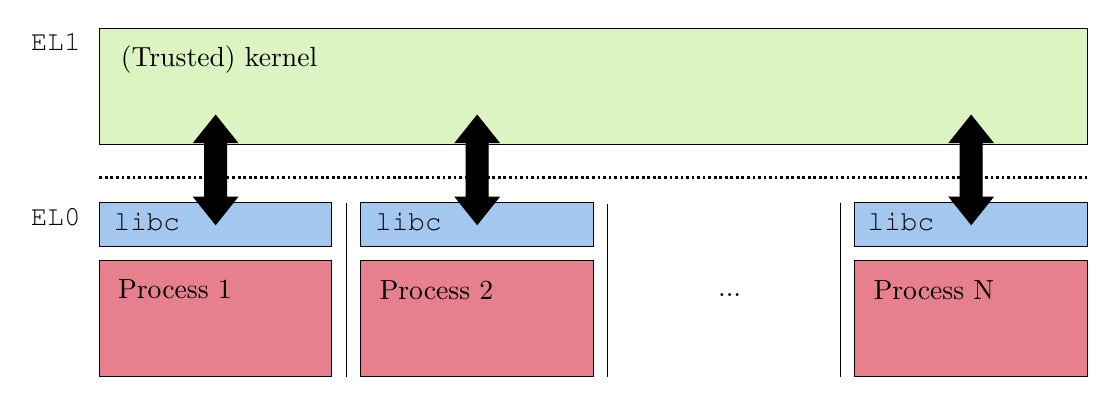
\begin{tikzpicture}[x=0.75pt,y=0.75pt,yscale=-0.7,xscale=0.7]
%uncomment if require: \path (0,300); %set diagram left start at 0, and has height of 300

%Straight Lines [id:da0238858095373361] 
\draw [line width=1]  [dash pattern={on 1pt off 1pt}]  (10,133) -- (690,133) ;
%Shape: Rectangle [id:dp18633003951104476] 
\draw  [fill={rgb, 255:red, 184; green, 233; blue, 134 }  ,fill opacity=0.5 ] (10,30) -- (690,30) -- (690,110) -- (10,110) -- cycle ;
%Straight Lines [id:da8836005156472156] 
\draw    (180,150) -- (180,270) ;
%Straight Lines [id:da0871105771687758] 
\draw    (360,151) -- (360,270) ;
%Straight Lines [id:da47486673087950704] 
\draw    (520,150) -- (520,270) ;
%Flowchart: Process [id:dp5014112861074582] 
\draw  [fill={rgb, 255:red, 208; green, 2; blue, 27 }  ,fill opacity=0.5 ] (10,190) -- (170,190) -- (170,270) -- (10,270) -- cycle ;
%Flowchart: Process [id:dp5474401833590941] 
\draw  [fill={rgb, 255:red, 208; green, 2; blue, 27 }  ,fill opacity=0.5 ] (190,190) -- (350,190) -- (350,270) -- (190,270) -- cycle ;
%Flowchart: Process [id:dp05943677937308278] 
\draw  [fill={rgb, 255:red, 208; green, 2; blue, 27 }  ,fill opacity=0.5 ] (530,190) -- (690,190) -- (690,270) -- (530,270) -- cycle ;
%Flowchart: Process [id:dp22719106375428721] 
\draw  [fill={rgb, 255:red, 74; green, 144; blue, 226 }  ,fill opacity=0.5 ] (10,150) -- (170,150) -- (170,180) -- (10,180) -- cycle ;
%Flowchart: Process [id:dp418634561741007] 
\draw  [fill={rgb, 255:red, 74; green, 144; blue, 226 }  ,fill opacity=0.5 ] (190,150) -- (350,150) -- (350,180) -- (190,180) -- cycle ;
%Flowchart: Process [id:dp5808126324898445] 
\draw  [fill={rgb, 255:red, 74; green, 144; blue, 226 }  ,fill opacity=0.5 ] (530,150) -- (690,150) -- (690,180) -- (530,180) -- cycle ;
%Left Right Arrow [id:dp18252152506193997] 
\draw  [fill={rgb, 255:red, 0; green, 0; blue, 0 }  ,fill opacity=1 ] (90,90) -- (105,108.75) -- (97.5,108.75) -- (97.5,146.25) -- (105,146.25) -- (90,165) -- (75,146.25) -- (82.5,146.25) -- (82.5,108.75) -- (75,108.75) -- cycle ;
%Left Right Arrow [id:dp937447124008122] 
\draw  [fill={rgb, 255:red, 0; green, 0; blue, 0 }  ,fill opacity=1 ] (270,90) -- (285,108.75) -- (277.5,108.75) -- (277.5,146.25) -- (285,146.25) -- (270,165) -- (255,146.25) -- (262.5,146.25) -- (262.5,108.75) -- (255,108.75) -- cycle ;
%Left Right Arrow [id:dp43564214029042536] 
\draw  [fill={rgb, 255:red, 0; green, 0; blue, 0 }  ,fill opacity=1 ] (610,90) -- (625,108.75) -- (617.5,108.75) -- (617.5,146.25) -- (625,146.25) -- (610,165) -- (595,146.25) -- (602.5,146.25) -- (602.5,108.75) -- (595,108.75) -- cycle ;

% Text Node
\draw (23,40) node [anchor=north west][inner sep=0.75pt]   [align=left] {{\fontfamily{rm}\selectfont (Trusted) kernel}};
% Text Node
\draw (434,211) node [anchor=north west][inner sep=0.75pt]   [align=left] {{\fontfamily{rm}\selectfont ...}};
% Text Node
\draw (18,155) node [anchor=north west][inner sep=0.75pt]   [align=left] {{\fontfamily{pcr}\selectfont libc}};
% Text Node
\draw (198,155) node [anchor=north west][inner sep=0.75pt]   [align=left] {{\fontfamily{pcr}\selectfont libc}};
% Text Node
\draw (537,155) node [anchor=north west][inner sep=0.75pt]   [align=left] {{\fontfamily{pcr}\selectfont libc}};
% Text Node
\draw (21,201) node [anchor=north west][inner sep=0.75pt]   [align=left] {{\fontfamily{rm}\selectfont Process 1}};
% Text Node
\draw (201,202) node [anchor=north west][inner sep=0.75pt]   [align=left] {{\fontfamily{rm}\selectfont Process 2}};
% Text Node
\draw (541,202) node [anchor=north west][inner sep=0.75pt]   [align=left] {{\fontfamily{rm}\selectfont Process N}};
% Text Node
\draw (-39,32) node [anchor=north west][inner sep=0.75pt]   [align=left] {{\fontfamily{pcr}\selectfont EL1}};
% Text Node
\draw (-39,152) node [anchor=north west][inner sep=0.75pt]   [align=left] {{\fontfamily{pcr}\selectfont EL0}};
\end{tikzpicture}
\caption{A schematic of the typical system organization of a commodity operating system and its associated user-space.
The kernel (in green) executes at a relative level of privilege compared to user-space (red) enforced by hardware---here, we follow the Arm convention and show the kernel executing at \texttt{EL1} and user-space at \texttt{EL0}.
The two communicate across a system call boundary (dashed line) using system calls (black arrows), with user-space typically making use of a library such as \texttt{libc} (blue) to abstract over this process.}
\label{fig.operating-system.schematic}
\end{figure}

Most commodity operating systems---that is, Microsoft Windows and Unix-derivatives\footnote{To guard against quibbling over research operating systems like exokernels and similar which can be argued not to fit this pattern}---fit a common pattern and are architected around a relatively self-contained, trusted component typically called the system \emph{kernel}.

At system initialisation, the kernel takes control of all system resources.
Thereafter, untrusted user-space applications wishing to make use of a device, for example, must pass through the kernel in order to do so, which can either choose to gate or allow access.
Moreover, the kernel introduces a process abstraction in user-space, and the kernel tasks itself with ensuring that processes are always isolated from each other.
The kernel is therefore \emph{the} key component responsible for enforcing system-wide policies.
It is therefore imperative that the kernel is able to isolate itself sufficiently from untrusted user-space software at all times.

To help the kernel self-isolate, modern microprocessors are equipped with a number of features dedicated to this task.
One key feature are \emph{exception levels}\footnote{This is Arm-specific terminology.  \emph{Privilege rings} are the analogous feature on Intel platforms} which introduce a notion of \emph{privilege} into the system.
Here, software executing at a relative level of privilege---for example, an operating system kernel---is allowed to program sensitive system registers, controlling how the system operates, and ``peer in'' and potentially modify the runtime state of software executing at a lower-level of privilege.
The kernel may read data from, or write data to, a buffer ostensibly within the memory space of an untrusted user-space process, for example.
In this sense, a kernel can ``supervise'' or ``watch over'' untrusted user-space.

Moreover, modern microprocessors also provide a form of memory management built around page tables.
These data structures are used for virtualisation of the system memory---granting user-space software the illusion that they own the entire physical address space---and also for memory access and permissions checks.
By correctly initialising and managing these page tables the kernel's own data structures and scratch space can be kept isolated from untrusted user-space, and user-space processes can be kept isolated from each other.

Note that for systems software, isolation is therefore enforced by low-level machine mechanisms: namely separate address spaces, private parts of memory, and machine-enforced privilege checks on executing software.

Finally the kernel, by necessity, must expose a limited interface to untrusted user-space, which can be used to request access to system resources, or make other similar requests for intercession by the kernel.
To do this, operating system kernels commonly exposes a suite of \emph{system calls} to untrusted user-space, which can be invoked with dedicated machine instructions.
On Arm platforms---with which the author is most familiar---these instructions induce a processor exception, which causes a \emph{context switch} into the kernel, which handles the system call appropriately, before exiting the exception and returning the flow of program control back to the calling user-space program.
In this respect, from user-space's point-of-view, system calls have the appearance of very CISC-like machine instructions, and the operating system kernel essentially presents itself as ``silicon by other means''.

For all of this to work, user-space and the kernel must work together, and adopt a common calling convention describing how arguments and results are passed back-and-forth across the system call interface, agree on a binary interface detailing how system calls are identified and errors are reported, and so on and so forth.
However, crucially, it is \emph{generally} not the case that the operating system kernel and untrusted user-space applications need be written in the same programming language for this all to work.
Whilst most operating system kernels are written in some C-language derivative, user-space programs can be written in a variety of languages, and can all make use of system resources exposed by the kernel's system call interface as long as they are capable of adhering to the calling convention and binary interface expected by the kernel.
Whilst---on Linux at least\footnote{Note that this is not the case on some variants of BSD Unix, for example Apple MacOS, which generally consider the programming interface of the system C library as the interface of the kernel, proper}---this system call interface is abstracted over by the C library, \texttt{libc}, this is generally just a convenience, and user-space software can always invoke system calls directly if wanted by invoking the correct machine instruction and adhering to the appropriate calling convention.
In this respect, the C-language may have prominence of the favoured language of system implementation, but by-and-large it is not \emph{special} or given an unduly prominent status by the kernel itself.

\subsection{On programmable proof-checkers}

\begin{figure}
\tikzset{every picture/.style={line width=0.75pt}} %set default line width to 0.75pt        
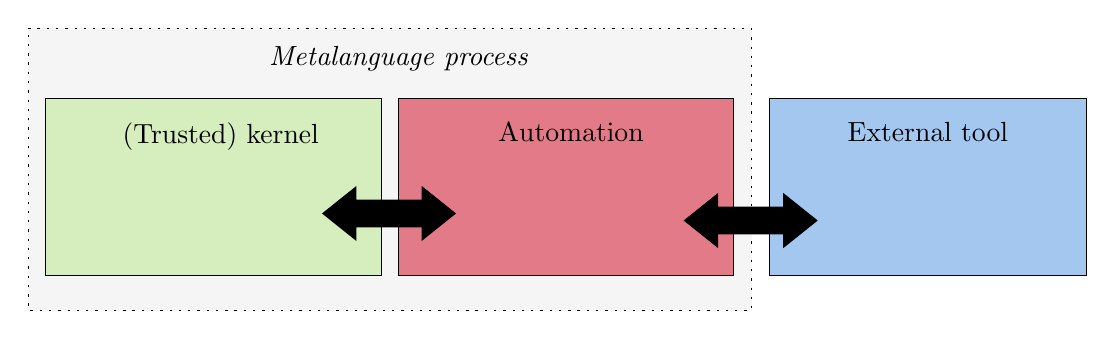
\begin{tikzpicture}[x=0.75pt,y=0.75pt,yscale=-0.85,xscale=0.85]
%uncomment if require: \path (0,300); %set diagram left start at 0, and has height of 300

%Shape: Rectangle [id:dp5145169571980753] 
\draw  [fill={rgb, 255:red, 155; green, 155; blue, 155 }  ,fill opacity=0.1 ][dash pattern={on 0.84pt off 2.51pt}] (10,10) -- (420,10) -- (420,170) -- (10,170) -- cycle ;
%Shape: Rectangle [id:dp7336028259076729] 
\draw  [fill={rgb, 255:red, 184; green, 233; blue, 134 }  ,fill opacity=0.5 ] (20,50) -- (210,50) -- (210,150) -- (20,150) -- cycle ;
%Shape: Rectangle [id:dp32707998554431983] 
\draw  [fill={rgb, 255:red, 208; green, 2; blue, 27 }  ,fill opacity=0.5 ] (220,50) -- (410,50) -- (410,150) -- (220,150) -- cycle ;
%Shape: Rectangle [id:dp3433596839522859] 
\draw  [fill={rgb, 255:red, 74; green, 144; blue, 226 }  ,fill opacity=0.5 ] (430,50) -- (610,50) -- (610,150) -- (430,150) -- cycle ;
%Left Right Arrow [id:dp2058390242799486] 
\draw  [fill={rgb, 255:red, 0; green, 0; blue, 0 }  ,fill opacity=1 ] (177,115) -- (195.75,100) -- (195.75,107.5) -- (233.25,107.5) -- (233.25,100) -- (252,115) -- (233.25,130) -- (233.25,122.5) -- (195.75,122.5) -- (195.75,130) -- cycle ;
%Left Right Arrow [id:dp5651724135135525] 
\draw  [fill={rgb, 255:red, 0; green, 0; blue, 0 }  ,fill opacity=1 ] (382,119) -- (400.75,104) -- (400.75,111.5) -- (438.25,111.5) -- (438.25,104) -- (457,119) -- (438.25,134) -- (438.25,126.5) -- (400.75,126.5) -- (400.75,134) -- cycle ;

% Text Node
\draw (145,19) node [anchor=north west][inner sep=0.75pt]   [align=left] {{\fontfamily{rm}\selectfont {\it Metalanguage process}}};
% Text Node
\draw (62,62) node [anchor=north west][inner sep=0.75pt]   [align=left] {{\fontfamily{rm}\selectfont (Trusted) kernel}};
% Text Node
\draw (275,62) node [anchor=north west][inner sep=0.75pt]   [align=left] {{\fontfamily{rm}\selectfont Automation}};
% Text Node
\draw (473,62) node [anchor=north west][inner sep=0.75pt]   [align=left] {{\fontfamily{rm}\selectfont External tool}};
\end{tikzpicture}
\caption{A schematic of the system organisation of a typical LCF-style proof assistant.
The trusted kernel (green) is linked against untrusted automation (red) existing within the same metalanguage process (dotted line) and communicate with each other using the kernel's API (black arrow).
External tools existing as separate processes (blue, must communicate with a shim layer written in the proof assistant's metalanguage to access the kernel (black arrow).}
\label{fig.proof-assistant.organization}
\end{figure}

Most modern proof assistants---that is, systems in the wider HOL family, Coq, Matita, PRL, and similar---fit a common pattern and are architected around a relatively self-contained, trusted component typically called the system \emph{kernel}.

The system kernel is the sole component that can authenticate claims as legitimate theorems of the implemented logic.
Untrusted automation, residing outside of the kernel, must ``drive'' the kernel to derive a theorem on its behalf.
The kernel is therefore \emph{the} component responsible for ensuring system-wide soundness.
It is therefore imperative that the kernel is able to isolate itself sufficiently from untrusted automation at all times.
This method of system organisation is known as \emph{the LCF approach} after the system which introduced it, and is the most common way of organising proof-checking systems today.

Most modern proof assistants tend to be written in a ``metalanguage'', typically a strongly-typed functional programming language, for example an ML derivative such as OCaml or SML.
These types of programming language offer strong modularity and abstraction features, which the kernel exploits to hide its own data structures from untrusted automation and expose a carefully limited API for proof-construction and manipulation.
Notably, in an LCF-style system, the \emph{only} mechanism automation has for constructing an authenticated theorem is by using this API, with the inference (or typing) rules of the logic exposed as ``smart constructors'' manipulating an abstract type of theorems or well-typed terms.

Untrusted automation and the system kernel are linked together, and reside side-by-side in the same process when the system is executed.
As a result, system soundness ultimately rests on the soundness of the implementation metalanguage's type-system---specifically its ability to correctly isolate module-private data structures, that is its ability to correctly enforce type abstraction.
Moreover, the system metalanguage is, in a sense, unique amongst all programming languages, in that it is the only language capable of interfacing with the kernel, which is, after all, ``just'' a module written within that language like any other.
Whilst external tools, and automation written in other languages, can interface with the kernel, it must do so indirectly, making use of a shim layer written in the system metalanguage.

\subsection{The Supervisionary system}

In many respects, as the text above intimates, the role of the kernel in an operating system and the role of the kernel in a proof-checker is, abstractly, \emph{essentially} the same.
Namely, both components must enforce system-wide invariants in the face of---and correctly isolate themselves from---unbridled interaction with untrusted code.
However, the two mechanisms through which these different types of kernel self-isolate are very different: for operating system kernels\footnote{Barring unikernels like Mirage, which are in some respects quite similar to LCF-style proof-checkers in this regard} self-isolation is enforced using machine-oriented mechanisms; for LCF-style proof-checkers, self-isolation is enforced using programming language-oriented mechanisms.

In this paper we introduce \emph{Supervisionary}, a novel programmable proof-checker for Gordon's HOL whose design will be further discussed in detail in Section~\ref{sect.kernel.design}.
(Note that many of the ideas presented henceforth are logic-independent, and though we have chosen to use HOL in our prototype, can be applied to a wide array of other logics with minimal changes.)
Of note, Supervionary's system design has more in common with the typical system organisation of an operating system than comparable implementations of HOL.
Specifically, the Supervisionary kernel executes at a relative level of privilege when compared to untrusted automation, which can be thought of as executing in something akin to Supervisionary's version of ``user space''.
The trusted kernel, and untrusted user space, communicate across a system call boundary, which must be carefully designed in order to ensure system soundness.

One immediate consequence of this design is that the Supervisionary kernel immediately takes on a very different character to the typical LCF kernel.
Specifically, all of the typical paraphernalia of a HOL implementation---type formers, types, constants, terms, and theorems---are kept safely under the management of the Supervisionary kernel itself, in private memory areas, and never exposed directly to user-space but rather referenced indirectly by handles.
These handles may be thought of as somewhat akin to pointers into Supervisionary's private memories, or analogous to file handles in typical systems software, and are used by user-space software to denote a kernel object that the Supervisionary kernel should manipulate or query on user-space's behalf.

Remarkably, Supervisionary is also not implemented in a typed functional programming language, as is typical of most programmable proof-checkers, but rather in the \emph{unsafe} systems programming language, Rust.
Note that this implementation decision introduces no risk to system soundness which ultimately rests on the separation of kernel-private data from user-space, using privilege and private memories, not on programming language features.
Moreover, as user-space and kernel communicate across a defined system call interface, untrusted user-space may also be written in \emph{any} programming language capable of producing code that is binary-compatible with the Supervisionary kernel.
Supervisionary therefore has no ``metalanguage'' in the sense understood by users of LCF-style provers, but rather an implementation language, with automation potentially written in multiple languages.

We implement Supervisionary as a WebAssembly (or Wasm, henceforth) host.
This allows us to experiment with the essential ideas behind Supervisionary---namely isolating the kernel using private memory areas, which the ``user-space'' Wasm program executing under the host cannot access, and which exposes services via system call-like interface---without become bogged down in extraneous detail associated with booting a real machine, and interacting with real hardware.
Moreover, we harness work on porting compiler and linker toolchains, allowing our ``user space'' to be written in any language capable of targeting Wasm.

\section{Kernel design}
\label{sect.kernel.design}

\subsection{Implemented logic}

Supervisionary implements a variant of Gordon's HOL, a classical higher-order logic which can be intuitively understood as Church's Simple Theory of Types extended with ML-style top-level polymorphism.
We introduce the basics of this logic here, introducing just enough material so that the unfamiliar reader can follow the rest of the paper.

We fix a set of \emph{type variables} and use $\alpha$, $\beta$, $\gamma$, and so on, to range arbitrarily over them.
With these, we work with a grammar of \emph{types} generated by the following recursive grammar:
\begin{gather*}
\tau, \tau', \tau'' ::= \alpha \mid \mathsf{f}(\tau, \ldots, \tau')
\end{gather*}
Here $\mathsf{f}$ is a \emph{type-former} which has an associated \emph{arity}---a natural number indicating the number of type arguments that it expects.
If all type-formers within a type are applied to their expected number of types we call the type \emph{well-formed}---that is, arities introduce a trivial or degenerate form of \emph{kinding} for types.
We will only ever work with well-formed types in Supervisionary.
We write $tv(\tau)$ for the \emph{set of type-variables} appearing within a type, and write $\tau[\alpha := \tau']$ for the \emph{type substitution} replacing all occurrences of $\alpha$ with $\tau'$ in the type $\tau$.
From the outset we assume two primitive type-formers---essentially built-in to the logic itself, and necessary to bootstrap the rest of the logic: $\mathsf{bool}$, the type-former of the Boolean type (and in HOL, also propositions), with arity $0$, and $- \Rightarrow -$, the type-former of the HOL function space, with arity $2$.
Note we will abuse syntax and also write $\mathsf{bool}$ for the \emph{type} of Booleans and propositions, and also write $\tau \Rightarrow \tau'$ for the function space type.

For each well-formed type $\tau$ we assume a countably infinite set of \emph{variables} and \emph{constant symbols}.
We use $x_\tau$, $y_\tau$, $z_\tau$, and so on, to range over the variables associated with type $\tau$, and use $\mathsf{C}_\tau$, $\mathsf{D}_\tau$, $\mathsf{E}_\tau$, and so on, to also range over the constants associated with type $\tau$.
With these, we recursively define \emph{terms} of the explicitly-typed $\lambda$-calculus, as follows:
\begin{displaymath}
r, s, t ::= x_\tau \mid \mathsf{C}_\tau \mid rs \mid \lam{x{:}\tau}r
\end{displaymath}
Note that there is an ``obvious'' typing relation on terms, which we omit here, and we call any term with a type \emph{well-typed}.
We will only ever work with well-typed terms in Supervisionary, and call terms with type $\mathsf{bool}$ \emph{formulae}.
We will use $\phi$, $\psi$, $\xi$, and so on, to suggestively range over terms that should be understood as being formulae.
We work with terms up-to $\alpha$-equivalence, write $fv(r)$ for the set of \emph{free variables} appearing within the term $r$, write $r[x_\tau := t]$ for the usual \emph{capture-avoiding substitution} on terms, and write $r[\alpha := \tau]$ for the recursive extension of the type substitution action to terms.

Like with type-formers, from the offset we assume a collection of typed constants needed to boostrap the rest of the logic, summarised in the table below:
\begin{center}
\begin{tabular}{cc}
$=$ & $\alpha \Rightarrow \alpha \Rightarrow \mathsf{bool}$ \\
$\top$, $\bot$ & $\mathsf{bool}$ \\
$\neg$ & $\mathsf{bool} \Rightarrow \mathsf{bool}$ \\
$\wedge$, $\vee$, $\longrightarrow$ & $\mathsf{bool} \Rightarrow \mathsf{bool} \Rightarrow \mathsf{bool}$ \\
$\forall$, $\exists$ & $(\alpha \Rightarrow \mathsf{bool}) \Rightarrow \mathsf{bool}$ \\
$\epsilon$ & $(\alpha \Rightarrow \mathsf{bool}) \Rightarrow \mathsf{\alpha}$
\end{tabular}
\end{center}
The majority of the constants above correspond to the usual logical constants and connectives of first- or higher-order logic and are introduced without further explanation.
Only the latter $\epsilon$ constant---Hilbert's description operator, a form of choice---may be unfamiliar.
In HOL, this can be used to ``select'', or ``choose'' an element of a type according to some predicate, and is otherwise undefined if no such element exists.
Note that all HOL types are inhabited by at least one element.
We adopt usual mathematical conventions and precedence levels when writing terms making use of these constants, writing $\phi \longrightarrow \psi$ instead of $(\longrightarrow\ \phi)\psi$, for example.
We also suppress explicit type substitutions required to make terms involving polymorphic types well-typed, writing $\fall{x_\tau}\phi$ instead of $\forall[\alpha := \tau](\lam{x_\tau}\phi)$, for example.

We call a finite set of formulae a \emph{context}, ranged arbitrarily over by $\Gamma$, $\Gamma'$, $\Gamma''$, and so on, and introduce a two-place \emph{Natural Deduction relation} between contexts and formula using the rules in Figure~\ref{fig.natural.deduction}.
We write $\Gamma \vdash \phi$ to assert that a derivation tree rooted at $\Gamma \vdash \phi$ and constructed according to the rules presented in Figure~\ref{fig.natural.deduction} exists.

\begin{figure}
\begin{gather*}
\end{gather*}
\caption{The Natural Deduction relation for Gordon's HOL.}
\label{fig.natural.deduction}
\end{figure}

\subsection{The kernel state}

The Supervisionary kernel maintains several private \emph{heaps} containing \emph{kernel objects} of various kinds, corresponding to the various objects that constitute the HOL logic: type-formers, types, constants, terms, and theorems.

\subsection{The kernel system call interface}

\subsection{Programming the kernel}

\subsection{Specifying kernel functions}

\section{Capabilities on steroids}
\label{sect.capabilities.on.steroids}

\section{Conclusions}
\label{sect.conclusions}

\subsection{Related work}

\subsection{Future work}

\end{document}
